% AY2014 力学 解答例
% 体裁・粒度は 参考/ のPDFに揃える（行間を埋め、最終解答は \ans{} で boxed）。
% 解答・数値・問題は本年度過去問から自力で導いた（東大版は体裁の手本のみ）。
\documentclass[11pt,a4paper]{article}
\usepackage{../../../00_common/preamble}

\usetikzlibrary{decorations.pathmorphing}
\usetikzlibrary{calc}

\title{力学 AY2014 解答例（専門基礎科目）}
\author{}
\date{}

\begin{document}
\maketitle

% ==================================================================
\section*{第1問〔I〕}

質量 $m$ の質点が長さ $a$ の軽い糸につながれ，点 O を中心として反時計回りに
一定の角速度 $\omega$ で回転している。重力は無視する。
質点の位置を $\bm{r}(t)=(a\cos\omega t,\ a\sin\omega t)$ と表すと，
質点は半径 $a$ の等速円運動を行う。

\begin{center}
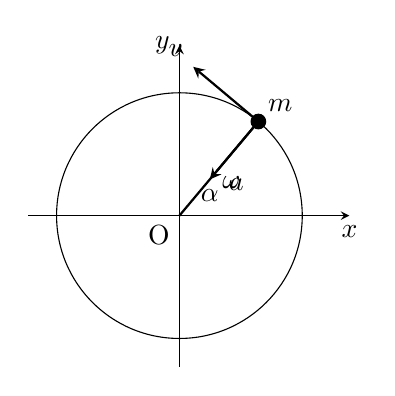
\begin{tikzpicture}[>=stealth, scale=1.2]
  \draw[->] (-1.6,0)--(1.8,0) node[below]{$x$};
  \draw[->] (0,-1.6)--(0,1.8) node[left]{$y$};
  \draw[thin] (0,0) circle (1.3);
  \node[below left] at (0,0) {O};
  % 質点（角度 50度付近）
  \coordinate (P) at (50:1.3);
  \draw[thick] (0,0)--(P) node[midway,below right]{$a$};
  \draw[fill=black] (P) circle (2.2pt);
  \node[above right] at (P) {$m$};
  % 速度（接線方向，反時計回り）
  \draw[->,thick] (P)--($(P)+(140:0.9)$) node[above left]{$\bm{v}$};
  % 加速度（中心向き）
  \draw[->,thick] (P)--($(P)+(230:0.8)$) node[below]{$\bm{\alpha}$};
  \node at (0.55,0.35) {$\omega$};
\end{tikzpicture}

{\small 反時計回りの等速円運動。$\bm{v}$ は接線向き，$\bm{\alpha}$ は中心 O 向き}
\end{center}

\subsection*{(1) 速度の大きさと向き}
位置 $\bm{r}=(a\cos\omega t,\ a\sin\omega t)$ を時間微分して
\begin{align*}
  \bm{v}=\dot{\bm{r}}=(-a\omega\sin\omega t,\ a\omega\cos\omega t).
\end{align*}
大きさは
\[
  |\bm{v}|=\sqrt{(a\omega\sin\omega t)^2+(a\omega\cos\omega t)^2}=a\omega.
\]
また $\bm{r}\cdot\bm{v}=-a^2\omega\sin\omega t\cos\omega t+a^2\omega\cos\omega t\sin\omega t=0$
より $\bm{v}\perp\bm{r}$ であり，速度は糸に垂直な接線方向（回転の向き，すなわち反時計回り）を向く。
\[
  \ans{\;|\bm{v}|=a\omega,\quad \text{向きは糸に垂直な接線方向（反時計回り）}\;}
\]

\subsection*{(2) 加速度の大きさと向き}
速度をさらに時間微分して
\begin{align*}
  \bm{\alpha}=\dot{\bm{v}}=(-a\omega^2\cos\omega t,\ -a\omega^2\sin\omega t)=-\omega^2\bm{r}.
\end{align*}
大きさは
\[
  |\bm{\alpha}|=\omega^2|\bm{r}|=a\omega^2.
\]
$\bm{\alpha}=-\omega^2\bm{r}$ は位置ベクトルと逆向き，すなわち中心 O に向かう向き（向心加速度）である。
\[
  \ans{\;|\bm{\alpha}|=a\omega^2,\quad \text{向きは中心 O に向かう向き（向心方向）}\;}
\]

\subsection*{(3) 1 周の間に張力がする仕事}
糸の張力 $\bm{T}$ は糸に沿って中心 O へ向かう向き，すなわち $\bm{r}$ と逆向きである。
一方 (1) より速度 $\bm{v}$ は $\bm{r}$ に垂直であるから，常に $\bm{T}\perp\bm{v}$ となる。
よって瞬間仕事率は
\[
  \bm{T}\cdot\bm{v}=0
\]
であり，1 周（$0\le t\le 2\pi/\omega$）にわたって積分しても
\[
  W=\int_{0}^{2\pi/\omega}\bm{T}\cdot\bm{v}\,dt=0.
\]
\[
  \ans{\;W=0\;}
\]
（張力は向心方向の力で運動方向に成分をもたないため，仕事をしない。
実際 $|\bm{v}|=a\omega$ は一定で運動エネルギーは変化せず，仕事が $0$ であることと整合する。）

\subsection*{(4) 角運動量の保存}
原点 O まわりの角運動量は $\bm{L}=\bm{r}\times m\bm{v}$。質点に働く力は糸の張力のみで，
これは中心 O を向く中心力 $\bm{T}=-T\,\hat{\bm{r}}$（$\hat{\bm{r}}=\bm{r}/a$）である。
よって O まわりの力のモーメントは
\begin{align*}
  \bm{N}=\bm{r}\times\bm{T}=\bm{r}\times\bigl(-T\,\hat{\bm{r}}\bigr)
   =-\frac{T}{a}\,(\bm{r}\times\bm{r})=\bm{0}.
\end{align*}
角運動量の時間変化は $\dfrac{d\bm{L}}{dt}=\bm{N}=\bm{0}$ であるから $\bm{L}$ は一定，
すなわち角運動量は保存される。
実際に成分計算すると（$z$ 成分のみ）
\begin{align*}
  L_z&=m(x v_y-y v_x)\\
   &=m\bigl[a\cos\omega t\cdot a\omega\cos\omega t-a\sin\omega t\cdot(-a\omega\sin\omega t)\bigr]
    =m a^2\omega,
\end{align*}
となり時間によらず一定である。
\[
  \ans{\;\dfrac{d\bm{L}}{dt}=\bm{r}\times\bm{T}=\bm{0}\ \therefore\ \bm{L}=m a^2\omega\ (\text{一定})\;}
\]

\medskip
検算: (1)(2) より向心加速度 $a\omega^2$ に質量を掛けると向心力 $m a\omega^2$ を得る。
これは張力 $T$ そのものであり，運動方程式 $T=m a\omega^2$ と一致する。
また (4) の $|\bm{L}|=ma^2\omega=m\,a\cdot(a\omega)=m\,a\,|\bm{v}|$ は，
「半径 $\times$ 運動量」に等しく次元・大きさとも妥当。✓

% ==================================================================
\clearpage
\section*{第2問〔II〕}

一辺 $L$ の立方体容器中に $n$ モルの単原子理想気体が入っている。
気体分子の質量を $m$，$i$ 番目の分子の速度を
$\bm{v}_i=(v_{ix},\,v_{iy},\,v_{iz})$ とする。分子は壁と完全弾性衝突し，
分子同士の衝突は無視する。壁 A は $x=L$ にある $yz$ 面に平行な壁である。

\subsection*{(1) 1 回の衝突で壁が受ける力積}
壁 A は $x$ に垂直であるから，完全弾性衝突では $x$ 方向の速度成分のみ符号反転し，
$y,z$ 成分は変わらない。衝突前 $v_{ix}\,(>0)$，衝突後 $-v_{ix}$ より，
分子の運動量の $x$ 成分の変化は
\begin{align*}
  \Delta p_{x}=m(-v_{ix})-m v_{ix}=-2m v_{ix}.
\end{align*}
作用反作用より壁が受ける $x$ 方向の力積は，この符号を反転した
\[
  J=-\Delta p_x=2m v_{ix}.
\]
\[
  \ans{\;J=2m v_{ix}\ (\text{$+x$ 向き})\;}
\]

\subsection*{(2) 1 秒間に壁 A に衝突する回数}
$x$ 方向には速さ $v_{ix}$ で往復する。壁 A に衝突してから次に壁 A に衝突するまでには
$x$ 方向に往復で距離 $2L$ を進む。所要時間は $\dfrac{2L}{v_{ix}}$ であるから，
1 秒間の衝突回数は
\[
  f=\frac{1}{\,2L/v_{ix}\,}=\frac{v_{ix}}{2L}.
\]
\[
  \ans{\;f=\dfrac{v_{ix}}{2L}\;}
\]

\subsection*{(3) $i$ 番目の分子が壁 A に加える力}
1 秒間に壁が受ける力積の総和が，壁が受ける（時間平均の）力に等しい。
(1)(2) より
\begin{align*}
  F_i=J\cdot f=2m v_{ix}\cdot\frac{v_{ix}}{2L}=\frac{m v_{ix}^2}{L}.
\end{align*}
\[
  \ans{\;F_i=\dfrac{m v_{ix}^2}{L}\;}
\]

\subsection*{(4) $n$ モル全分子が壁 A に加える力}
分子の総数は $N=n N_A$ 個。全分子からの力は (3) の和であり，
$x$ 方向速度の 2 乗平均 $\langle v_x^2\rangle=\dfrac{1}{N}\sum_{i=1}^{N}v_{ix}^2$ を用いると
\begin{align*}
  F=\sum_{i=1}^{N}\frac{m v_{ix}^2}{L}
   =\frac{m}{L}\sum_{i=1}^{N}v_{ix}^2
   =\frac{m}{L}\,N\langle v_x^2\rangle
   =\frac{n N_A m\langle v_x^2\rangle}{L}.
\end{align*}
\[
  \ans{\;F=\dfrac{n N_A m\langle v_x^2\rangle}{L}\;}
\]

\subsection*{(5) $E=\dfrac{3}{2}nRT$ の導出}
壁 A の面積は $L^2$ であるから，壁にかかる圧力は (4) より
\begin{align*}
  P=\frac{F}{L^2}=\frac{n N_A m\langle v_x^2\rangle}{L^3}
   =\frac{n N_A m\langle v_x^2\rangle}{V},
\end{align*}
ここで体積 $V=L^3$ を用いた。よって
\begin{align*}
  PV=n N_A m\langle v_x^2\rangle.
\end{align*}
等方性 $\langle v_x^2\rangle=\dfrac{1}{3}\langle v^2\rangle$ を代入すると
\begin{align*}
  PV=\frac{1}{3}n N_A m\langle v^2\rangle.
\end{align*}
これを状態方程式 $PV=nRT$ と等置して
\begin{align*}
  nRT=\frac{1}{3}n N_A m\langle v^2\rangle
  \quad\therefore\quad
  N_A m\langle v^2\rangle=3RT.
\end{align*}
一方，全分子の運動エネルギーは（単原子分子なので並進のみ）
\begin{align*}
  E=\sum_{i=1}^{N}\frac{1}{2}m v_i^2
   =\frac{1}{2}m\,N\langle v^2\rangle
   =\frac{1}{2}m\,(n N_A)\langle v^2\rangle
   =\frac{1}{2}n\,\bigl(N_A m\langle v^2\rangle\bigr).
\end{align*}
ここに $N_A m\langle v^2\rangle=3RT$ を代入すると
\begin{align*}
  E=\frac{1}{2}n\cdot 3RT=\frac{3}{2}nRT.
\end{align*}
\[
  \ans{\;E=\dfrac{3}{2}nRT\;}
\]

\medskip
検算: 1 分子あたりの平均並進運動エネルギーは
$\dfrac{E}{N}=\dfrac{(3/2)nRT}{n N_A}=\dfrac{3}{2}\dfrac{R}{N_A}T=\dfrac{3}{2}k_B T$
（$k_B=R/N_A$ はボルツマン定数）となり，エネルギー等分配則
（並進 3 自由度 $\times\frac12 k_B T$）と一致する。✓

\end{document}
